\chapter{Iteration 3}
\label{ch:iter3}

The third iteration of \textbf{HiringGuru} was planned for completion around the midterm of FYP-2. This chapter outlines the core design and testing activities conducted during this phase, focusing on the structural and behavioral aspects of the system. While the functional requirements remained consistent, the system architecture evolved to support a robust, scalable, and maintainable real-time mock interview platform with integrated AI-based analysis.

\section{Structural Design}

\subsection{Domain Model/Class Diagram}
The domain model defines key entities in the HiringGuru ecosystem, including \texttt{User}, \texttt{Interview}, \texttt{AnalysisResults}, and \texttt{Feedback}. The class diagram illustrates the interaction among components of the Node.js backend, Next.js frontend, and AI modules, showcasing the object-oriented structure of the application.

\subsection{Component Diagram}
The component diagram presents a modular breakdown of HiringGuru’s architecture. It includes:
\begin{itemize}
  \item Backend (Node.js + Express)
  \item Frontend (Next.js + TailwindCSS)
  \item AI Modules: MobileNetV2 (posture detection), MediaPipe (landmark analysis), Haarcascade (facial expression), Dlib (eye tracking)
  \item External APIs: OpenAI for question generation
  \item Database: Firebase Realtime Database
\end{itemize}
These components are designed to work asynchronously and in real-time to ensure a smooth user experience.

\subsection{Layer Diagram}
HiringGuru is structured in a layered architecture:
\begin{itemize}
  \item \textbf{Presentation Layer:} Next.js with TailwindCSS
  \item \textbf{Business Logic Layer:} Node.js backend handling APIs and middleware
  \item \textbf{AI Analysis Layer:} TensorFlow, OpenCV (CV2), MediaPipe, Dlib
  \item \textbf{Data Access Layer:} Firebase Realtime Database
\end{itemize}

\subsection{Structure Chart}
The structure chart showcases the hierarchical module organization: from the core interview engine and voice synthesis module (Python TTS) to AI-based analytics modules, including posture and facial tracking subsystems. The AI modules achieve over 90\% accuracy in posture analysis.

\section{Behavior Design}

\subsection{Flow Diagram}
The flow diagram depicts the end-to-end user journey, beginning with Firebase-based authentication, progressing through the interview session, AI-powered analysis, and real-time feedback presentation.

\subsection{Data Flow Diagram (DFD)}
The DFD visualizes how webcam input is processed:
\begin{itemize}
  \item Captured via browser
  \item Converted to grayscale using CV2
  \item Fed into trained AI models (e.g., MobileNetV2, MediaPipe)
  \item Results are stored in Firebase and displayed via the frontend
\end{itemize}

\subsection{Data Dictionary}
The data dictionary defines elements such as:
\begin{itemize}
  \item \texttt{User}: \texttt{name}, \texttt{email}, \texttt{role}
  \item \texttt{Interview}: \texttt{sessionId}, \texttt{timestamp}, \texttt{questions}
  \item \texttt{AnalysisResults}: posture accuracy, facial expression score, eye tracking metrics
  \item \texttt{Feedback}: timestamp, suggestions, scores
\end{itemize}

\subsection{Activity Diagram}
The activity diagram demonstrates the interview process lifecycle:
\begin{enumerate}
  \item Session initialization
  \item Dynamic question generation via OpenAI API
  \item Real-time AI analysis and user monitoring
  \item Feedback generation and session summary
\end{enumerate}

\subsection{State Machine Diagram}
The state machine tracks session transitions, such as:
\begin{itemize}
  \item \texttt{Idle} → \texttt{Recording} (user starts interview)
  \item \texttt{Recording} → \texttt{Analyzing} (frame-by-frame AI analysis)
  \item \texttt{Analyzing} → \texttt{Feedback} (session ends, data summarized)
\end{itemize}

\subsection{Sequence Diagram}
The sequence diagram details interactions between:
\begin{itemize}
  \item Next.js frontend
  \item Node.js backend API
  \item Firebase Database
  \item TensorFlow and Python-based AI scripts
\end{itemize}
This flow ensures minimal latency during real-time analysis.

\subsection{Interaction Overview Diagram}
A high-level integration of activity and sequence diagrams, showing how frontend UI triggers backend processes, feeds into AI models, and synchronizes data with Firebase for feedback display.

\section{Schema Design / ER Diagram}
The ER diagram maps Firebase collections and their attributes, including:
\begin{itemize}
  \item \texttt{Users}: UID, Email, Role
  \item \texttt{Interviews}: InterviewID, Timestamp, UserID
  \item \texttt{AnalysisResults}: InterviewID, FrameMetrics, TimeLogs
  \item \texttt{Feedback}: InterviewID, Suggestions, Final Scores
\end{itemize}

\section{Data Structure Design}
Key data structures include:
\begin{itemize}
  \item \textbf{Arrays:} Frame-wise AI results
  \item \textbf{Objects:} User sessions, interview metadata
  \item \textbf{Dictionaries/Maps:} Real-time feedback and error handling
\end{itemize}

\section{Algorithm Design}
HiringGuru incorporates multiple AI algorithms:
\begin{itemize}
  \item \textbf{Posture Analysis:} MobileNetV2 achieving ~90\% accuracy
  \item \textbf{Face Tracking:} Haarcascade classifiers
  \item \textbf{Eye Movement:} Dlib-based shape prediction
  \item \textbf{Question Generation:} OpenAI GPT-based prompts
\end{itemize}

\section{Development Phase}
\begin{itemize}
  \item \textbf{Coding Standards:} ESLint and Prettier for Node.js/Next.js
  \item \textbf{Styling:} TailwindCSS for consistency and responsiveness
  \item \textbf{Static Analysis:} Integration of linters and testing tools
\end{itemize}

\subsection{Unit Tests}
\begin{table}[!htbp]
\centering
\begin{tabular}{|c|p{8cm}|c|}
\hline
\textbf{Test Case ID} & \textbf{Description} & \textbf{Expected Output} \\
\hline
UT-01 & Validate OpenAI API returns relevant question set & Accurate questions displayed \\
\hline
UT-02 & Ensure AI posture analysis handles bad frames & Graceful fallback, no crash \\
\hline
\end{tabular}
\caption{Sample Unit Test Cases}
\label{tab:unit-test-cases}
\end{table}

\subsection{Test Suites}
Test suites include:
\begin{itemize}
  \item Functional Testing: Core interview features
  \item Integration Testing: Backend-AI-Firebase communication
  \item Regression Testing: Post feature addition
\end{itemize}

\section{Maintainable Phase}

\subsection{CI/CD}
CI/CD pipeline is integrated with GitHub Actions:
\begin{itemize}
  \item Automated builds and test execution
  \item Deployment to Vercel (frontend) and Firebase (backend + DB)
\end{itemize}

\subsection{Deployment Diagram}
The deployment diagram shows:
\begin{itemize}
  \item Next.js frontend hosted on Vercel
  \item Node.js backend deployed via Firebase Functions
  \item Firebase Realtime Database for persistent storage
  \item External AI scripts running on local Python services
\end{itemize}

\subsection{System-Level Tests}
\begin{table}[!htbp]
\centering
\begin{tabular}{|c|p{8cm}|c|}
\hline
\textbf{Test Case ID} & \textbf{Description} & \textbf{Expected Output} \\
\hline
ST-01 & End-to-end login and session initiation & Successful login and interview load \\
\hline
ST-02 & Data storage for every second/frame & Data logged and stored in Firebase \\
\hline
\end{tabular}
\caption{System-Level Test Cases}
\label{tab:system-test-cases}
\end{table}

\subsection{GitHub Repository}
All source code and documentation are maintained in the following GitHub repository:  
\textbf{\url{https://github.com/12Samad/FYP-HiringGuru}}

\subsection{Setup and Tool Manual}
HiringGuru setup requires:
\begin{itemize}
  \item Node.js, Next.js, and TailwindCSS
  \item Python 3.x with TensorFlow, OpenCV, MediaPipe, Dlib
  \item Firebase project setup and environment configuration
  \item OpenAI API key for dynamic question generation
\end{itemize}

\section{UML Use Case Diagram}
\begin{figure}[h]
  \centering
  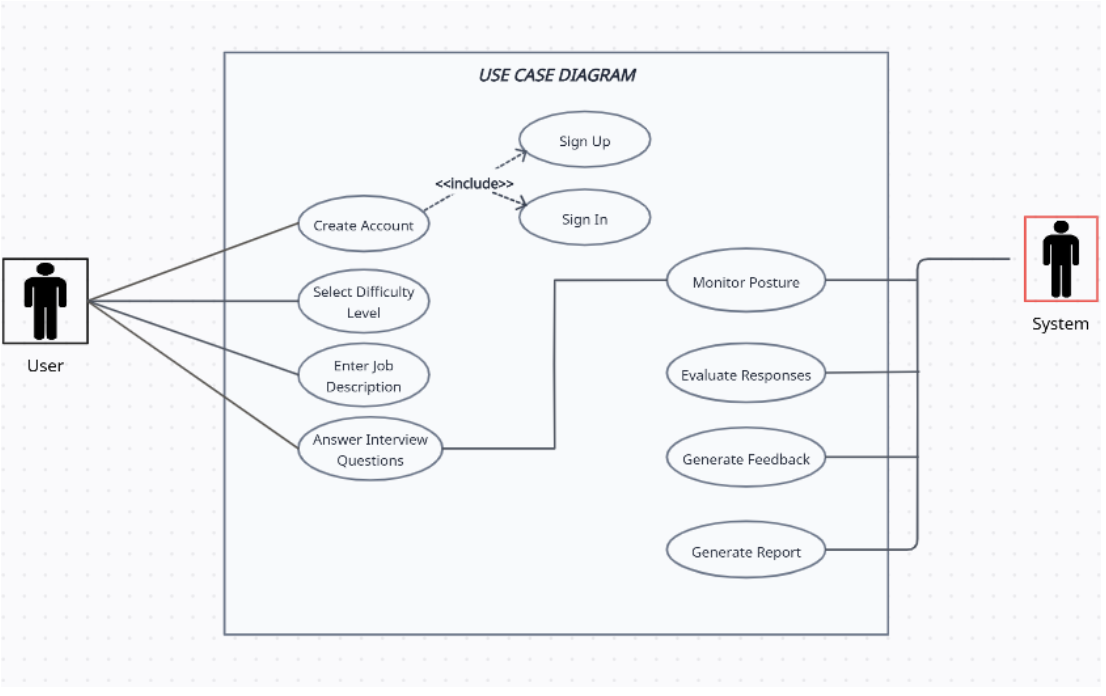
\includegraphics[width=0.8\textwidth]{sections/diagrams/UseCase.png}
  \caption{UML Use Case Diagram for HiringGuru}
  \label{fig:use-case}
\end{figure}

This chapter documents the design, implementation, and testing strategies that contributed to a functional and scalable version of HiringGuru by Iteration 3. The combination of web technologies and AI modules has laid a solid foundation for continued development and refinement of the real-time mock interview platform.

